\documentclass[a4]{seminar}

\usepackage{palatino,epsfig}

\def\N{\mathsf{l\kern -.15em N}}
\def\Z{\mathsf{Z\kern -.4em Z}}
\def\Q{\mathsf{l\kern -.35em Q}}
\def\eqdef{\mathrel{\smash{\mathop{\kern 0pt{=}}\limits^{\hbox{\tiny def}}}}}
\def\depij{\mathrel{\smash{\mathop{\kern 0pt{\longrightarrow}}\limits^{\theta_i^j,\omega_i^j}}}}
\newtheorem{claim}{Claim}
\newtheorem{lemma}{Lemma}
\newtheorem{theorem}{Theorem}
\newtheorem{property}{Property}
\newtheorem{corollary}{Corollary}
\newtheorem{definition}{Definition}
\def\proof{\par\noindent{\em Proof: }}
\def\endproof{\ \hfill\lower 1ex\vbox{\hrule\hbox{\vrule\phantom
    p\vrule}\hrule}\medskip}

\usepackage{slidesec}

\newslideframe{IMAGE}{%
  \boxput{\rput(1,0){\includegraphics[scale=0.4]{st}}}{#1}}
\slideframe*{IMAGE}

\usepackage{pstcol} % To use the standard `color' package with Seminar
\usepackage{semcolor}
\usepackage{slidesec}
\input{seminar.bug}
\input{seminar.bg2} % See the Seminar bugs list

\usepackage{graphicx}
\usepackage{fancybox}

\usepackage{fancyhdr}
% Headers and footers personalization using the `fancyhdr' package
\fancyhf{} % Clear all fields
\renewcommand{\headrulewidth}{0.2mm}
\renewcommand{\footrulewidth}{0.2mm}
\fancyhead[L]{\small\textsf{A Machine Description System}}
\fancyhead[R]{\small\textsf{\theslideheading}}
%\fancyfoot[L]{\tiny\textsf\thedate}
\fancyfoot[L]{\scriptsize\textsf{April 12, 2005}}
\fancyfoot[R]{\scriptsize\textsf\theslide}
% To avoid that the headers be too close of the top of the page
\renewcommand{\slidetopmargin}{2cm}
% To center horizontally the headers and footers (see seminar.bug)
\renewcommand{\headwidth}{\textwidth}
% To adjust the frame length to the header and footer ones
\autoslidemarginstrue

\slideframe{none}

\begin{document}

\thispagestyle{empty}

\begin{slide}

\begin{center}

{\large\bf A Machine Description System \\
Status and Development Directions}

\vspace{15 mm}

{Beno\^{\i}t Dupont de Dinechin \\
%AST Embedded Systems Research Laboratory \\
%Via Cantonale 16E 6928 Manno Switzerland \\
\texttt{Benoit.Dupont-de-Dinechin@st.com}}

\vspace{5 mm}


\epsfig{file=EPS/stlogo.eps,width=20mm} {STMicroelectronics}

{\small April 12, 2005}

\end{center}

\end{slide}


\pagestyle{fancy}


\begin{slide}

\slideheading{Why a Machine Description System}

\begin{center} \underline{Software Development Tools Program Representations}
\end{center}

\begin{itemize}

\item Binary absolute and relocatable form

\item Assembler source and disassembler output

\item Assembler internal representation (instructions \& operands)

\item Compiler internal representation (operations \& parameters)

\end{itemize}

\begin{center} \underline{Software Development Tools ISA Representations}
\end{center}

\begin{itemize}

\item Binary encoding (operand, instructions, bundles)

\item Storage elements (memory, registers, constant generators)

\item Instruction behavior (instruction set simulation)

\item Instruction properties (compiler code optimizations)

\item Instruction semantics (compiler code selection)

\end{itemize}

\end{slide}


\begin{slide}

\begin{center} \underline{Purpose of a Machine Description System}
\end{center}

A Machine Description System (MDS) is a structured data repository and a
collection of programs used to configure the target-specific parts of the
software development tools.

\begin{center} \underline{Existing Machine Description Systems}
\end{center}

\begin{description}

\item[Green Hills Software] Canonical Machine Description to configure the
compiler, assembler, linker, disassembler, debugger.

\item[CMG Bristol Architects] CHESS tables to drive the documentation and the
instruction set simulator of the ST200 processors.

\item[Coware / LisaTek] Lisa language to automatically produce
simulators (instruction and cycle accurate), assembler, linker, debugger,
compiler instruction scheduler.

\end{description}

\end{slide}


\begin{slide}

\begin{description}

\item[U. of Virginia] Computer Systems Description Languages (CSDL). Different
languages and tools are available: SLED for encoding / decoding; RTL and
$\lambda$-RTL for instruction semantics; Alpha for calling conventions; Block
language for stack frame composition.

\item[Open64 TargInfo] Calls to a special C++ library to generate the Open64
target description tables and enumerations. This covers assembly syntax,
instruction encoding, bundling, scheduling, register allocation, ABI targeting.

\item[AST MachGen] C code \& data to configure the LxISS, the GNU AS, and to
generate constant evaluators for the LxBE.

\item[STS ARC \& CSD] Machine descriptions systems respectively used by the LAO
ST100 and the LAO ST200. The ARC covered assembly syntax, instruction encoding,
bundling, scheduling, register allocation, instruction properties and semantics.

\end{description}

\end{slide}


\begin{slide}

\begin{center} \underline{Lessons from these Machine Description Systems}
\end{center}

\begin{itemize}

\item The CSDL system from U. of Virginia is the most advanced, but is now a
disparate collection of language and tools.

\item The single language-based approaches (GHS, Lisa) mix the different
description levels and constrain the description into some hierarchy. A single
language cannot cover everything.

\item The authoring of machine descriptions in C++ (Open64 TargInfo, AST MachGen)
tends to be tool-centric so they do not include the descriptions they don't use.

\item Not able to describe aliases between storage locations (Open64).

\item No instruction selection / peephole re-selection generators.

\item No understanding of instruction bundling / bundle templates.

\item Not able to distinguish between core-specific and target-specific.

\end{itemize}

\end{slide}


\begin{slide}

\slideheading{Design of the AST/STS MDS}

\begin{center} \underline{AST/STS MDS Design Objectives} \end{center}

In case of the AST/STS Machine Description System, we focus on:
\begin{itemize}

\item Assembling and disassembling, linking with the GNU tools.

\item Automatic generation of the Open64 TargInfo source code.

\item Automatic generation of the LAO2 target description tables.

\item Replacement of some MachGen capabilities for the AST ISS.

\item High-speed instruction and bundle encoding for the AST X-JIT.

\item Eventually able to describe stack frames and ABI conventions.

\item Describe all the ST200 cores; next describe ARM cores (V5E).

\end{itemize}

\end{slide}


\begin{slide}

\begin{center} \underline{AST/STS MDS Design Decisions} \end{center}

\begin{itemize}

\item Focus on the completeness, the non-redundancy, and the verifiability, of
the MDS data repository:
  \begin{itemize}
    \item use a pseudo-relational data schema (allows embedded lists)
    \item encode data repository as XML and validate against DTD
    \item use mini-languages in XML element contents and parse them
  \end{itemize}

\item Organize MDS processing in three stages:
  \begin{itemize}
    \item front-end processing to translates and enrich foreign machine
    descriptions into the MDS data repository;
    \item central part that expands information, merge identical core-level
    information into target-level information, and validates contents;
    \item back-end processing to generate the files needed by each software
    development tool.
  \end{itemize}

\end{itemize}

\end{slide}


\begin{slide}

\begin{center} \underline{AST/STS MDS Design Decisions (Continued)} \end{center}

\begin{itemize}

\item Ensure compiler-level information is available:
  \begin{itemize}
    \item Multiple calling conventions and register roles for each
    \item Register files and register classes for register allocation
    \item Instruction scheduling information that is core specific
    \item Use internal Behavior language to extract compiler properties
  \end{itemize}

\item Ensure VLIW instruction bundling can be described:
  \begin{itemize}
    \item Instruction bundling of VLIW processors does not fit in a
    variable-length instruction framework!
    \item Instruction scheduling must produce valid bundles!
    \item View VLIW bundle encoding as a two-step process: encode
    variable-length instruction; recode the encoded instructions and add control
    bits to make bundle
  \end{itemize}

\end{itemize}

\end{slide}


\begin{slide}

\begin{center} \underline{Why Use XML for MDS Data Repository} \end{center}

\begin{itemize}

\item Text information repository under revision control

\item Easily convertible to specification documents

\item Stable lexical structure (escapes, macros, inclusion)

\item User-defined information structure (DTD)

\item Standard validation and processing tools (OpenSP)

\end{itemize}

\begin{center} \underline{Common XML Mistakes to Avoid} \end{center}

\begin{itemize}

\item Lack of overall structure of the XML database

\item Encode every bit of document structure in XML

\item Use of unproven XML technologies (XML Schema validation)

\end{itemize}

\begin{center} \fbox{We only use DTD validation, pseudo-relational tables,
and plain Perl} \end{center}

\end{slide}


\begin{slide}

\begin{center} \underline{Example of XML DTD Fragment} \end{center}

{\small
\begin{verbatim}
<!ELEMENT Immediate EMPTY>
<!ATTLIST Immediate
  ID            ID              #REQUIRED
  what          CDATA           #IMPLIED
  name          NMTOKEN         #REQUIRED
  size          NMTOKEN         #REQUIRED
  shift         NMTOKEN         #IMPLIED
  bias          NMTOKEN         #IMPLIED
  extend        ( Signed        |
                  Unsigned )    #REQUIRED
  relative      ( PC            |
                  GP )          #IMPLIED
  relocation    NMTOKEN         #IMPLIED
>
\end{verbatim}
}

\end{slide}


\begin{slide}

\begin{center} \underline{Corresponding XML Fragment} \end{center}

{\small
\begin{verbatim}
<Immediate
  ID=   "Immediate:ST200:BTARG"
  name= "BTARG"
  relative=     "PC"
  shift=        "2"
  size= "23"
  extend= "Signed"
/>
<Immediate
  ID=   "Immediate:ST200:ISRC2"
  name= "ISRC2"
  size= "9"
  extend= "Signed"
/>
\end{verbatim}
}

\end{slide}


\begin{slide}

\slideheading{Implementation of the AST/STS MDS}

\begin{description}

\item[June 2004] Initial prototype of the MDS by Benoit.

\item[July -- August 2004] Stephen Clarke generates the GNU AS tables.

\item[August 2004] Benoit forks the MDS into MDS2 to configure and build the MDS
tables for simultaneous cores.

\item[September 2004] Stephen Clarke generates most of the Open64 TargInfo files
except scheduling and ABI information and contributes a decode tree generator.

\item[October -- November 2004] Benoit generalizes the MDS core process
and implements a Behavior language compiled from Takumi.

\item[February -- March 2005] Stephen Clarke finalizes MDS generation for
production Open64 and GNU assembler / disassembler.

\item[March -- April 2005] Benoit sets CodeX MDS and generates for LAO.

\end{description}

\end{slide}


\begin{slide}

\begin{center} \underline{AST/STS MDS Organization and Flows} \end{center}

\begin{itemize}

\item Available under \texttt{http://mds.codex.cro.st.com/}

{\scriptsize
\begin{verbatim}
svn co https://svn.mds.codex.cro.st.com/svnroot/mds/trunk/MDS
mkdir build && cd build
../MDS/configure --target=st200 --with-cores="st235" --enable-tools="gnu o64"
make clean all check diff
\end{verbatim}
}

\item Front-end scripting creates the Machine Description Database (MDD) XML
tables from a variety of non-XML sources (CHESS, MachGen, special scripts)

\item The MDD XML tables are expanded using target-independent scripts into
Machine Description Expanded (MDE) XML tables; then the target-level
tables are merged across the different cores

\item Back-end scripting processes the MDS (MDD+MDE) XML tables and produce the
files needed by software development tools:  GNU AS tables, Open64 TargInfo, LAO
machine description, etc.

\end{itemize}

\end{slide}


\begin{slide}

\begin{center}
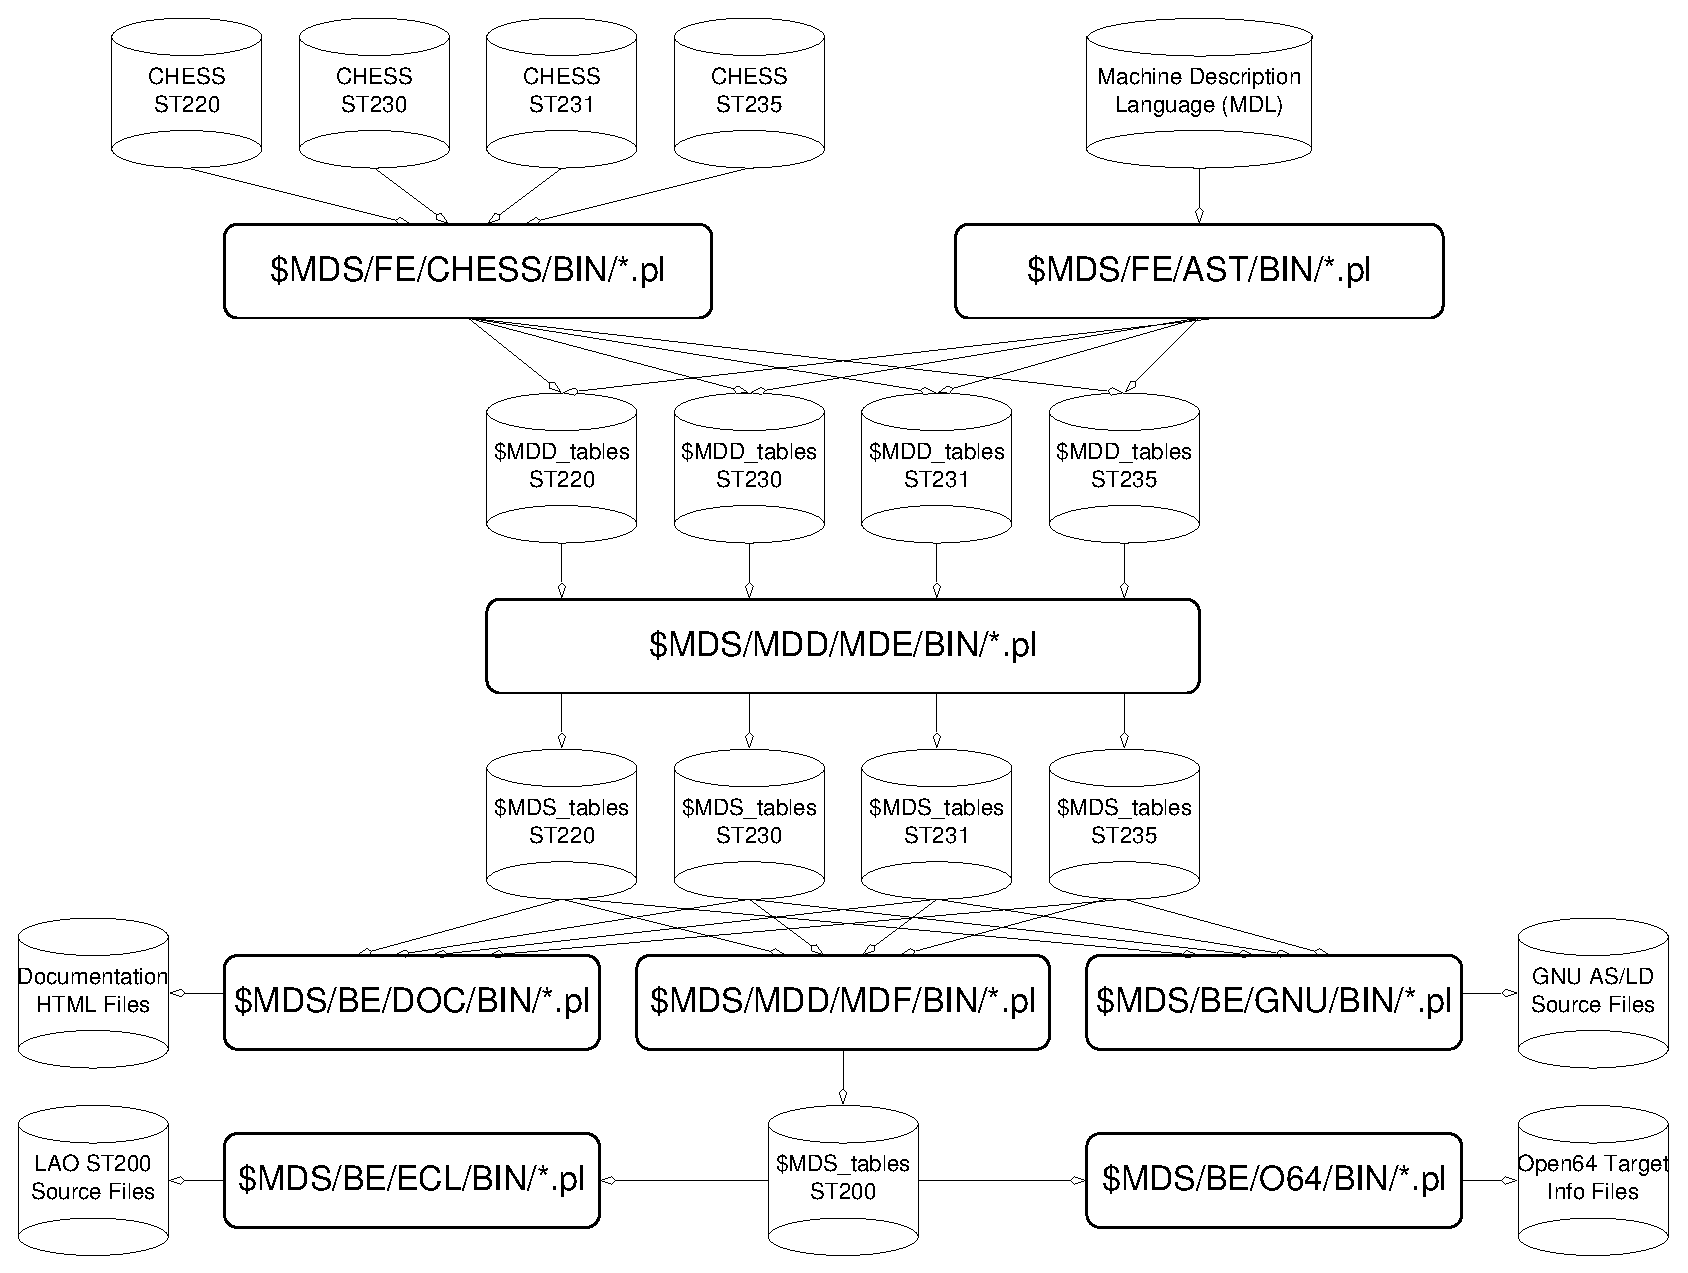
\epsfig{file=FIG/mds-flow.eps,width=100mm}
\end{center}

\end{slide}


\begin{slide}

\begin{center} \underline{MDS Documentation} \end{center}

\begin{itemize}

\item The bulk of the documentation is in the \verb|$MDS/DOC/MDD.dtd| DTD
file that explain the purpose of each XML element.

\item This commented DTD file is turned into LaTeX files then included into
the \verb|$MDS/DOC/Design.tex| file. Do \verb|make doc| in the \verb|build|
directory to build the documentation.

\item Grammars for the MDS mini-languages are included: \verb|$MDS/DOC/Takumi.y|
for the CHESS Takumi language; \verb|$MDS/DOC/Behavior.y| and
  \verb|$MDS/DOC/Semantics.y| for the MDS behavior and semantics languages.

\end{itemize}

\begin{center} \underline{MDS Auxiliary Tools} \end{center}

A parser generator in Perl for Bison grammars is included in
\verb|$MDS/BIN/yaxcc.pl|. See documentation embedded in that file.

\end{slide}


\begin{slide}

\slideheading{MDS Design Outline}

\begin{description}

\item[Storage] The machine memory, register files, control registers, constant generators.

\item[BitField] Identify a contiguous range of bits in a word.

\item[Operand] Variant part of an Instruction encoding associated with an
encoding method: Immediate, Modifier, RegClass, RegMask.

\item[Pattern] Bit pattern as a list of BitField(s) and expected values.

\item[Format] Specification for encoding Instruction(s) with a particular
operand list and provides the corresponding assembler syntax.

\item[Convention] Calling convention, including the register roles.

\item[Processor] High-level scheduling features of a processor.

\item[Register] Architectural register (MDE).

\end{description}

\end{slide}


\begin{slide}

\begin{center} \underline{Instruction XML Specification} \end{center}

An instruction is a member of the ISA not yet specialized with regards to the
operand list. Operand lists are defined by the Instruction \texttt{formats}.

{\scriptsize
\begin{verbatim}
<!ELEMENT Instruction (Behavior?)>
<!ATTLIST Instruction
  ID            ID              #REQUIRED
  what          CDATA           #IMPLIED
  mnemonic      NMTOKEN         #REQUIRED
  formats       IDREFS          #REQUIRED
  classes       IDREFS          #REQUIRED
  patterns      IDREFS          #REQUIRED
  syntax        CDATA           #IMPLIED
  specialize    IDREFS          #IMPLIED
  replacement   IDREFS          #IMPLIED
  synthetic     IDREF           #IMPLIED
  semantics     CDATA           #IMPLIED
>
\end{verbatim}
}

\end{slide}


\begin{slide}

\begin{center} \underline{ST235 ANDC Instruction} \end{center}

{\scriptsize
\begin{verbatim}
<Instruction
  ID=   "Instruction:st235:ANDC"
  classes=      "Scheduling:st235:ALU Scheduling:st235:ALU Scheduling:st235:ALUX"
  formats=      "Format:st235:Int3R Format:st235:Int3I Format:st235:Int3I.X"
  mnemonic=     "andc"
  patterns=     "Pattern:st200:andc.st235"
><Behavior
  proxies=      "%1 %2 %3"
>
(SEQ
  (WRITE..result1
    (AND
      (NOT
        (SX.32
          (READ.2.%2)))
      (SX.32
        (READ.2.%3))))
  (WRITE.3.%1
    (READ..result1)))
</Behavior></Instruction>
\end{verbatim}
}

\end{slide}


\begin{slide}

\begin{center} \underline{Opcode XML Specification} \end{center}

An instruction Opcode results from the database join of Instruction and
Format. In the corresponding Behavior, the access to operands is specialized.

{\scriptsize
\begin{verbatim}
<!ELEMENT Opcode (Behavior?)>
<!ATTLIST Opcode
  ID            ID              #REQUIRED
  instruction   IDREF           #REQUIRED
  mnemonic      NMTOKEN         #REQUIRED
  operands      IDREFS          #IMPLIED
  format        IDREF           #REQUIRED
  syntax        CDATA           #REQUIRED
  scheduling    IDREF           #REQUIRED
  bundling      IDREF           #IMPLIED
  decoding      IDREF           #REQUIRED
  patterns      IDREFS          #REQUIRED
  encoded       NMTOKEN         #REQUIRED
>
\end{verbatim}
}

\end{slide}


\begin{slide}

\begin{center} \underline{ST235 ANDC Opcode Register--Register--Register} \end{center}

{\scriptsize
\begin{verbatim}
<Opcode
  ID=   "Opcode:st235:ANDC_DEST_SRC1_SRC2"
  bundling=     "Bundling:st200:ALU"
  decoding=     "Decoding:st235:ANY"
  encoded=      "-0000001010000------------------"
  format=       "Format:st235:Int3R"
  instruction=  "Instruction:st235:ANDC"
  mnemonic=     "andc"
  operands=     "Operand:st200:DEST Operand:st200:SRC1 Operand:st200:SRC2"
  patterns=     "Pattern:st200:Int3R.st235 Pattern:st200:RESERVED_30_1 Pattern:st200:RESERVED_18_3 Pattern:st200:andc.st235"
  scheduling=   "Scheduling:st235:ALU"
  syntax=       "%0 %1 = %2, %3"
><Behavior
  methods=      "RegClass:st200:General RegClass:st200:General RegClass:st200:General"
  proxies=      "%1 %2 %3"
>
\end{verbatim}
}

\end{slide}


\begin{slide}

\begin{center} \underline{ST235 ANDC Opcode Register--Register--Register (Continued)} \end{center}

{\scriptsize
\begin{verbatim}
(SEQ
  (WRITE..result1
    (AND
      (NOT
        (F2S.32
          (LOAD.2.GR
            (METHOD.%2)
            (CONST.1))))
      (F2S.32
        (LOAD.2.GR
          (METHOD.%3)
          (CONST.1)))))
  (STORE.3.GR
    (METHOD.%1)
    (CONST.1)
    (I2F
      (CONST.32)
      (READ..result1))))
</Behavior></Opcode>
\end{verbatim}
}

\end{slide}


\begin{slide}

\begin{center} \underline{Operator XML Specification} \end{center}

An Operator is the compiler abstraction of an instruction Opcode.

Unlike Opcode, an Operator has Parameter(s) instead of Operand(s).

There is exactly one Parameter per Read or Write action of the Operator (not
accounting for side-effects on State Storage), independently from the Operand
encoding issues.

{\scriptsize
\begin{verbatim}
<!ELEMENT Operator (Parameter*, Semantics?)>
<!ATTLIST Operator
  ID            ID              #REQUIRED
  cores         NMTOKENS        #IMPLIED
  opcodes       IDREFS          #IMPLIED
  simulated     IDREFS          #IMPLIED
  attributes    NMTOKENS        #IMPLIED
  operands      IDREFS          #IMPLIED
  mnemonic      NMTOKEN         #REQUIRED
  syntax        CDATA           #REQUIRED
>
\end{verbatim}
}

\end{slide}

\begin{slide}

\begin{center} \underline{ST200 ANDC Operator Register--Register--Register} \end{center}

{\scriptsize
\begin{verbatim}
<Operator ID=   "Operator:st200:ANDC_DEST_SRC1_SRC2"
  cores=        "st220 st230 st231 st235"
  opcodes=      "Opcode:st220:ANDC_DEST_SRC1_SRC2 Opcode:st230:ANDC_DEST_SRC1_SRC2 Opcode:st231:ANDC_DEST_SRC1_SRC2 Opcode:st235:ANDC_DEST_SRC1_SRC2"
  mnemonic=     "andc"
  operands=     "Operand:st200:DEST Operand:st200:SRC1 Operand:st200:SRC2"
  syntax=       "%0 %1 = %2, %3"
><Parameter
  action=       "Write"
  method=       "RegClass:st200:General"
  proxy=        "%1"
  stages=       "3 3 3 3"
/><Parameter
  action=       "Read"
  method=       "RegClass:st200:General"
  proxy=        "%2"
  stages=       "2 2 2 2"
/><Parameter
  action=       "Read"
  method=       "RegClass:st200:General"
  proxy=        "%3"
  stages=       "2 2 2 2"
\end{verbatim}
}

\end{slide}


\begin{slide}

\begin{center} \underline{MDS Behavior Language} \end{center}

\begin{itemize}

\item The Behavior language is based on statements and captures common
sub-expressions in temporary variables.

\item It has control-flow constructs but no looping nor recursion.

\item Computations use with infinite precision or boolean arithmetic and
explicitly cast from/to bit-fields when accessing storage.

\end{itemize}

\begin{center} \underline{MDS Semantics Language} \end{center}

\begin{itemize}

\item The Semantics language is a parallel list of guarded computations, where
all the sub-expressions have been forward-substituted.

\item All computations work on bit-field type annotated with the minimum bit
precision required for correctness.

\item Not yet (used for compiler properties and instruction selection)

\end{itemize}

\end{slide}


\begin{slide}

\slideheading{Future Work}

\begin{center} \underline{MDS Short-Term Developments} \end{center}

\begin{itemize}

\item Merge the Semantics language and tools by Christophe Guillon

\item Produce the LAO ST200 target tables for the ST235 64-bit pairs

\item Target the MDS to the ARM architecture: first target is V5E (no Thumb)

\item More factored information into Format, including Behavior of Operand access

\item Develop a PseudoC language to describe Instruction behavior and compile
it into MDS Behavior

\item Design a Machine Description Language (MDL) to avoid authoring XML tables
by scripts

\end{itemize}

\end{slide}


\begin{slide}

\begin{center} \underline{MDS Mid-Term Developments} \end{center}

\begin{itemize}

\item Produce effective binary code compressors based on the bundle and
instruction encoding trees

\item Produce instruction behavior functions and decoding automaton for use by
simulators

\item Exploit operator semantics in compiler range analysis and SSA
optimizations

\item Exploit operator semantics in compiler instruction selection and peep-hole
optimizations

\item Drive register allocation from the MDS contents, including management of
aliased register files

\end{itemize}

\end{slide}


\begin{slide}

\slideheading{Conclusions}

\begin{itemize}

\item The MDS has already accumulated over one man-year of effort

\item The MDS is used in production for the ST200 STS software tools

\item The MDS is key to the AST/Computing SoC.NET project

\item The MDS will be used by AST/Computing Advanced Architecture Research (G.
Desoli)

\item No other architecture description system has core merging capabilities,
which are required for embedded processor families

\item No other architecture description system can produce such accurate
compiler information

\item The MDS could handle orther architectures and improve its end-user
interface, but this requires more resources

\end{itemize}

\end{slide}


\end{document}

